\documentclass[12pt]{report}
\usepackage{verbatim}
\usepackage{fullpage}
\usepackage{etoolbox}
\usepackage{lipsum}
\usepackage{graphicx}
\usepackage{hyperref}
\usepackage{titlesec}
\usepackage{pdftexcmds}
\usepackage{minted}


\graphicspath{ {res/} }
\setcounter{secnumdepth}{4}
\titleformat{\paragraph}
{\normalfont\normalsize\bfseries}{\theparagraph}{1em}{}
\titlespacing*{\paragraph}
{0pt}{3.25ex plus 1ex minus .2ex}{1.5ex plus .2ex}

\newcommand{\HRule}{\rule{\linewidth}{0.5mm}}
\renewcommand\emph{\textbf}
\renewcommand{\baselinestretch}{1.1}

\newcommand{\printSQLtest}[1]
{
    \inputminted[linenos, breaklines, breakbytoken, tabsize=4, fontsize=\footnotesize]{mysql}{#1}
}

\newcommand{\printPHPImpl}[1]
{
    \inputminted[linenos, breaklines, breakbytoken, tabsize=4, fontsize=\footnotesize]{php}{#1}
}

\newcommand{\printPHP}[1]
{
    \printPHP{../www/php/#1}
}

\newcommand{\printSQLTablepage}[2]
{    
    \subsection{#2}
    \subsubsection{Code}
    \printSQLtest{../sql/parts/#1}
    \subsubsection{Explanation}
}

\begin{document}



\begin{titlepage}

    \center

    \textsc{\LARGE Universita' degli Studi di Messina}\\[0.1cm]
    \textsc{\Large Dipartimento di Matematica e Informatica}\\[0.5cm]
    \textsc{\Large Programming II project}\\[0.5cm]

    \HRule \\[0.4cm]
    { \huge \bfseries NetLayer}\\[0.1cm]

    {\large 11 June 2015}
    \HRule \\[1.5cm]

    \begin{minipage}{0.4\textwidth}
    \begin{flushleft} \large
    \emph{Authors:}\\
    Vittorio \textsc{Romeo}
    \end{flushleft}
    \end{minipage}
    ~
    \begin{minipage}{0.4\textwidth}
    \begin{flushright} \large
    \emph{Professors:} \\
    Massimo \textsc{Vilari}


    \end{flushright}
    \end{minipage}\\[4cm]

    \vfill


    \begin{minipage}{\linewidth}
        \centering
        \begin{minipage}{0.35\linewidth}
            \begin{figure}[H]
                \center
                
\includegraphics[width=2cm, height=2cm]{logovee}

                \url{http://vittorioromeo.info}
            \end{figure}
        \end{minipage}
        \hspace{0.27\linewidth}
        \begin{minipage}{0.35\linewidth}
            \begin{figure}[H]
                \center
                
\includegraphics[width=2cm, height=2cm]{logounime}

                \url{http://unime.it}
            \end{figure}
        \end{minipage}
    \end{minipage}\\[3cm]
\end{titlepage}



\pagenumbering{gobble}
\newcommand{\atoc}[1]{\addtocontents{toc}{#1\par}}
\renewcommand{\thesection}{\arabic{section}.}
\tableofcontents
\newpage
\pagenumbering{arabic}




\part{Project specifications}

    The following part of the document describes the project and its design/development process without exploring its implementation details.

    The part begins with a synthesis of the \emph{client request}. After a careful analysis of the request, a \emph{Software Requirements Specification} (SRS) was written.

    Writing a correct and informative SRS is of utmost importance to achieve an high-quality final product and ensuring the development process goes smoothly.

    The SRS will cover the following points in depth:

    \begin{itemize}
        \item \emph{Scope and purpose}.
        \item \emph{Feature and functions}.
        \item \emph{External interface requirements}.
        \item \emph{Functional requirements}.
        \item \emph{Example use cases}.
        \item \emph{Non-functional requirements}.
        \item \emph{Analysis models}.
    \end{itemize}

    \chapter{Client request}

        The client requests the design and implementation of an \emph{open-source multi-purpose C++14 networking library}. 

        The library must allow the client to develop its own \emph{server-client} architectures and applications with ease, while still being performant and allowing low-level operations if required.

        The client intends to use the library as a basis for the networking layer in applications belonging to different domains, ranging from \emph{chat web applications} to \emph{real-time games and simulations}.

        The library must fulfill the following requirements: 

        \begin{itemize}
            \item The library must be written in \emph{modern C++14}, making use of the latest features to improve performance, readability and flexibility.

            \item The library must target \emph{UNIX} systems, \emph{Windows} and \emph{MacOS}.

            \item The library must have a \emph{layered architecture}, allowing developers using it to go as low-level/high-level they desire.

            \item The library must deal with \emph{byte serialization} of native and user-defined classes. Nested serializable data structures must be supported. 

            \item The library must provide a generic \emph{tunnel abstraction} that represents a network entity providing and receiving data. A UDP socket tunnel implementation must be provided with the library.

            \item The library must provide an high-level abstraction for \emph{server-client} multithreaded architectures, allowing applications to asynchronously interact with any number of sockets and conveniently handle received packets via function dispatching.

            \item The library must provide metaprogramming facilities to generate and bind packet types at compile-time, allowing performant code generation for serialization/deserialization and communication.

            \item The library must be released under an \emph{open-source} license and promote collaboration and external contributions.
        \end{itemize}

        The client intends using the requested library \emph{to build platforms} for various projects, both for internal company usage and public usage.

        It is imperative for the library to be easily integrable with existing legacy system, such as architectures depending on relational databases.

        For ease of development and deployment, the client requested the library to be optionally usable in \emph{header-only} mode and compatibility with the \emph{CMake} build system.

        The abstraction provided by the library must work asynchronously by default, but an option to use blocking IO must be present. 

    \chapter{Software Requirements Specification}


        \section{Introduction}

            \subsection{Software engineering}

                \emph{Software engineering} is the study and an application of engineering to the design, development, and maintenance of software.

                The Bureau of Labor Statistics' definition is Research, design, develop, and test operating systems-level software, compilers, and network distribution software for medical, industrial, military, communications, aerospace, business, scientific, and general computing applications.

                Typical formal definitions of software engineering are:

                \begin{itemize}
                    \item The systematic application of scientific and technological knowledge, methods, and experience to the design, implementation, testing, and documentation of software.
                    \item The application of a systematic, disciplined, quantifiable approach to the development, operation, and maintenance of software.
                    \item An engineering discipline that is concerned with all aspects of software production.
                    \item The establishment and use of sound engineering principles in order to economically obtain software that is reliable and works efficiently on real machines.
                \end{itemize}   

                \subsubsection{Background}

                    The term \emph{software engineering} goes back to the '60s, when more complex programs started to be developed by teams composed by experts.

                    There was a radical transformation of software: from \emph{artisan product} to \emph{industrial product}.

                    A software engineer needs to be a good programmer, an algorithm and data structures expert with good knowledge of one or more programming languages.

                    He needs to know various design processes, must have the ability to convert generic requirements in well-detailed and accurate specifications, and needs to be able to communicate with the end-user in a language comprehensible to him comprehensible.

                    Software engineering, is, however, a discipline that's still evolving. There still are no definitive standards for the software development process.

                    Compared to traditional engineering, which is based upon mathematics and solid methods and where well-defined standards need to be followed, software engineering is greatly dependent on personal experience rather than mathematical tools.

                    Here's a brief history of software engineering:

                    \begin{itemize}
                        \item \emph{1950s}: Computers start to be used extensively in business applications.
                        \item \emph{1960s}: The first software product is marketed. 

                        IBM announces its unbundling in June 1969.
                        \item \emph{1970s}: Software products are now regularly bought by normal users. 

                        The software development industry grows rapidly despite the lack of financing.

                        The first software houses begin to emerge.
                    \end{itemize}

                \subsubsection{Differences with programming}

                    \begin{itemize}
                        \item A programmer writes a complete program.
                        \item A software engineer writes a software component that will be combined with components written by other software engineers to build a system.
                    \end{itemize}

                    \begin{itemize}
                        \item Programming is primarily a personal activity.
                        \item Software engineering is essentially a team activity.
                    \end{itemize}

                    \begin{itemize}
                        \item Programming is just one aspect of software development.
                        \item Large software systems must be developed similar to other engineering practices.
                    \end{itemize}

            \subsection{SRS}

                This \emph{Software Requirements Specification} (SRS) chapter contains all the information needed by software engineers and project managers to design and implement the requested forum creation/management framework.

                The SRS was written following the \emph{Institute of Electrical and Electronics Engineers} (IEEE) guidelines on SRS creation.

            \subsection{Purpose}
                The SRS chapter is contained in the \emph{non-technical} part of the thesis.

                Its purpose is providing a \emph{comprehensive description} of the objective and environment for the software under development.

                The SRS fully describes \emph{what the software will do} and \emph{how it will be expected to perform}.

            \subsection{Scope}

                \subsubsection{Identity}
                    The software that will be designed and produced will be called \emph{NetLayer}.

                \subsubsection{Feature extents}

                    The complete product will:

                    \begin{itemize}
                        \item Provide a library for the \emph{development of multi-purpose network applications and architectures}.
                        \item Provide abstractions for all the major  \emph{operating systems' networking layer}.
                        \item Provide an extensible and flexible  \emph{data serialization} module for primitive and user-defined classes.
                    \end{itemize}

                    NetLayer, however, will not be a complete framework for the development of applications. Every part of an application that does not deal with networking issues will not be covered by the product.

                \subsubsection{Benefits and objectives}

                    Development using NetLayer will give companies and individuals several benefits over \"from-scratch\" development.

                    \begin{itemize}
                        \item Usage of NetLayer will provide access to an \emph{easy-to-integrate} and \emph{easy-to-use} networking library.
                        \item Development and testing time will be \emph{significantly reduced}.
                        \item Code making use of the library will be \emph{modern, efficient and readable} thanks to C++14 features and abstractions.
                    \end{itemize}

        \section{General description}
            \subsection{Product perspective and functions}
                The product shares many basic aspects and features with existing networking libraries, improving upon them in the following ways:

                \begin{itemize}
                    \item A layer-based architecture allows developers to make use of both low-level constructs and operations and high-level abstractions in the same application.
                    \item The library will optionally allow developers to use a programming style similar to \emph{functional programming}, making use of callbacks and first-class functions to deal with packet management and function dispatching.
                    \item 
                \end{itemize}

            \subsection{User characteristics}
                NetLayer is targeted towards modern C++ developers experienced with C++11 and C++14 features. The library makes heavy use of modern metaprogramming paradigms and techniques - unfamiliar users will not be able to make full use of the library.

                A \"more functional\" interface is provided where possible, allowing users to use convenient abstractions for data serialization functions and networking functions.

                Familiarity with multithreading and synchronous computation is also required to use the library.

        \section{Glossary}

            The following list contains all the main elements that compose the architecture of NetLayer.

            \begin{itemize}
                \item \emph{Packet Buffer}: dynamically resizable buffer that can store and provide serialized generic data.
                \item \emph{Address}: union of an IP address and a port.
                \item \emph{Payload}: abstraction consisting of an Address and PcktBuf. It can be sent to and received by Tunnel instances.
                \item \emph{Tunnel}: abstraction of a Payload provider/receiver. The default Tunnel is an UDP socket. 
                \item \emph{Thread Safe Queue}: a lock-based thread safe queue that supports concurrent enqueueing and dequeueing.
                \item \emph{Managed Packet Buffer}: abstraction consisting of a Thread Safe Queue and a reference to a Tunnel. It can be either a \emph{Managed Receive Buffer}, which enqueues received data from the tunnel, or a \emph{Managed Send Buffer}, which enqueues data that will be sent through the tunnel.
                \item \emph{Managed Host}: union of an Address, a Tunnel, a Managed Receive Buffer and a Managed Send Buffer. Represents a network entity capable of sending and receiving data through a tunnel.
                \item \emph{Serializable}: abstraction over a tuple of generic types that automatically allows the user to serialize and deserialize data. Serializable packets can also be nested and contain dynamically-resizable data structures.
                \item \emph{Packet Bind}: compile-time bind of a Serializable to a Packet type. Used to generate a dispatch table.
                \item \emph{Dispatch Table}: compile-time function table that binds a function to specific packet binds. Used to handle received packets. 
                \item \emph{Context Managed Host}: union of a managed host and a dispatch table.
            \end{itemize}

        \section{Specific requirements}

            \subsection{External interface requirements}

                \emph{External interface requirements} identify and document the interfaces to other systems and external entities within the project scope.

                \subsubsection{User interfaces}
                    The product will not provide any graphical user interface. The users of the library will be able to access its functions and types using C++14.

                \subsubsection{Software interfaces}
                    The \emph{open-source policy} of NetLayer will allow its users to expand or improve existing functionality and to interact with other existing technologies.

            \subsection{Functional requirements}
                In software engineering, a \emph{functional requirement} defines a function of a system and its components.

                Functional requirements may be \emph{calculations}, \emph{technical details}, \emph{data manipulation and processing} and other specific functionality that define what a system is supposed to accomplish.

                Behavioral requirements describing all the cases where the system uses the functional requirements are captured in \emph{use cases}.

                \subsubsection{Packet management}
                    \begin{itemize}
                        \item \emph{Payloads and thread-safe queue}: an abstraction consisting of an address and data is provided, along with a thread-safe queue that is used for sending/receiving data to/from the network in managed buffers.
                        \item \emph{Managed buffers}: payloads will be enqueued and dequeued in managed buffers, that allow to asynchronously access the contents of their queue.
                    \end{itemize}

                    %%% TODO
                    %\begin{figure}[!htb]
                    %\caption{User/group hierarchy example.}
                    %\centering
                    %\includegraphics[width=0.5\textwidth]{ed/hier_user}
                    %\end{figure}

                 \subsubsection{Data serialization}
                    \begin{itemize}
                        \item \emph{Fundamental types}: fundamental C++ type serialization will automatically be provided by the library.                        
                        \item \emph{Common C++ classes}: serialization for commonly used C++ classes, such as \mintinline{cpp}{std::vector} and \mintinline{cpp}{std::array}, is provided by default.                         
                        \item \emph{Extensible serialization}: library user will be able to extend the serialization system with their own types, using simple class inheritance or macros for convenience.
                    \end{itemize}

                    %%% TODO
                    %\begin{figure}[!htb]
                    %\caption{Content hierarchy example.}
                    %\centering
                    %\includegraphics[width=1\textwidth]{ed/hier_sec}
                    %\end{figure}

                  \subsubsection{Tunnel management}
                    \begin{itemize}
                        \item \emph{Default tunnel: UDP}: a tunnel implementation, wrapping an UDP socket, is provided by default.
                        \item \emph{Default tunnel: mock}: a mock tunnel, for unit-testing purposes, is provided by default.
                        \item \emph{Tunnel interface}: an extensible tunnel interface is provided, allowing the users of the library to implement their own network tunnels.
                    \end{itemize}

                    %%% TODO
                    %\begin{figure}[!htb]
                    %\caption{Subscription/notification architecture example.}
                    %\centering
                    %\includegraphics[width=1\textwidth]{ed/hier_sub}
                    %\end{figure}

                \subsubsection{Context binding}
                 \begin{itemize}
                        \item \emph{Managed hosts}: abstraction consisting of a send managed buffer and a receive managed buffer. Allows the user to add processing threads and to poll the buffers for received data.
                        \item \emph{Dispatch table}: an extensible table, configurable at compile-time, is provided to allow the user to define functions which will automatically handle specific packet types. 
                        \item \emph{Context host}: union of a managed host and a dispatch table. Provides a convenient interface to quickly develop a server/client architecture capable of sending and receiving payloads.
                    \end{itemize}

            \newpage

%%% TODO %%%
            \subsection{Example use cases}
                In software and systems engineering, a \emph{use case} is a list of steps, typically defining interactions between one or more actors and a system, to achieve a goal.

                \subsubsection{Defining tunnel types}
                    ...
                    \paragraph{Actors}
                        \begin{itemize}
                            \item Developer.
                        \end{itemize}

                    \paragraph{Pre-conditions}
                        \begin{itemize}
                            \item
                        \end{itemize}

                    \paragraph{Flow of events}
                        \begin{itemize}
                            \item
                        \end{itemize}

                    \paragraph{Post-conditions}
                        \begin{itemize}
                            \item 
                        \end{itemize}

                \subsubsection{Defining serializable types}
                    ...
                    \paragraph{Actors}
                        \begin{itemize}
                            \item Developer.
                        \end{itemize}

                    \paragraph{Pre-conditions}
                        \begin{itemize}
                            
                        \end{itemize}

                    \paragraph{Flow of events}
                        \begin{itemize}
                            \item
                        \end{itemize}

                    \paragraph{Post-conditions}
                        \begin{itemize}
                            \item 
                        \end{itemize}

                \subsubsection{Binding types to dispatch table}
                    ...
                    \paragraph{Actors}
                        \begin{itemize}
                            \item Developer.
                        \end{itemize}

                    \paragraph{Flow of events}
                        \begin{itemize}
                            \item
                        \end{itemize}

                    \paragraph{Post-conditions}
                        \begin{itemize}
                            \item 
                        \end{itemize}
                \subsubsection{Defining a context host}
                    ...
                    \paragraph{Actors}
                        \begin{itemize}
                            \item Developer.
                        \end{itemize}

                \subsubsection{Handling incoming payloads}
                    ...
                    \paragraph{Actors}
                        \begin{itemize}
                            \item Developer.
                        \end{itemize}

                    \paragraph{Flow of events}
                        \begin{itemize}
                            \item
                        \end{itemize}

                    \paragraph{Post-conditions}
                        \begin{itemize}
                            \item 
                        \end{itemize}
                \subsubsection{Handling outgoing payloads}
                    ...
                    \paragraph{Actors}
                        \begin{itemize}
                            \item Developer.
                        \end{itemize}            

                    \paragraph{Flow of events}
                        \begin{itemize}
                            \item
                        \end{itemize}

                    \paragraph{Post-conditions}
                        \begin{itemize}
                            \item 
                        \end{itemize}
            %    \newpage
            
            \subsection{Non-functional requirements}
                Functional requirements are supported by \emph{non-functional requirements} (also known as quality requirements), which impose constraints on the design or implementation (such as performance requirements, security, or reliability).

                \subsubsection{Performance}
                    The system will be designed from the ground-up with emphasis on performance. As the forum may have huge amounts of contents and concurrent usage after its deployment, optimizing is a must.

                    When possible, functions will be implemented \emph{directly in the database}, for maximum performance.

                    Web backend functions will also be carefully \emph{optimized both for memory and speed}.

                \subsubsection{Reliability}
                    The system will have to be reliable and keep working in case of errors.

                    Database queries and functions will be executed in \emph{safe wrappers} that catch and handle errors carefully.

                \subsubsection{Security}
                    veeForum needs to guarantee privacy and security for users and administrator of the system.

                    Well-tested and well-received \emph{security idioms} and \emph{encryption algorithms} will have to be used throughout the implementation of the whole system.

                \subsubsection{Maintainability and portability}
                    Being an open-source project, \emph{maintainability}, \emph{extensibility} and \emph{portability} are key.

                    The code layer will be carefully designed and organized to allow easy maintenance, bugfixing and feature addition.

                    To ensure maximum portability, the product will be designed to work on the most popular \emph{GNU/Linux} distributions and will be thoroughly tested on different platforms.
        
        \section{Analysis models}
            \subsection{Activity diagrams}
                Activity diagrams are graphical representations of workflows of stepwise activities and actions with support for choice, iteration and concurrency. 
                In the Unified Modeling Language, activity diagrams are intended to model both computational and organisational processes (i.e. workflows). 
                Activity diagrams show the overall flow of control.

                \newpage

                The following diagram shows the steps that the \emph{forum management team} must take in order to setup and initialize a veeForum-enabled forum.

                \begin{figure}[H]
                \caption{Forum setup and initialization activity diagram.}
                \centering
                \includegraphics[width=1\textwidth]{uc/a1}
                \end{figure}

                \newpage

                The following diagram shows the steps required for \emph{user registration}

                \begin{figure}[H]
                \caption{User registration activity diagram.}
                \centering
                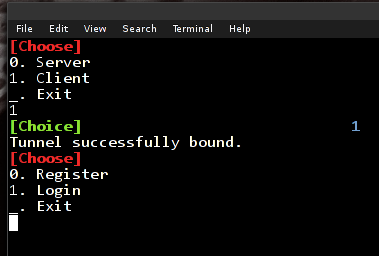
\includegraphics[width=0.65\textwidth]{di/1}
                \end{figure}

                \newpage

                The following diagram shows the steps required for \emph{user authentication}

                \begin{figure}[H]
                \caption{User authentication activity diagram.}
                \centering
                \includegraphics[width=1\textwidth]{di/8}
                \end{figure}

                \newpage

                The following diagrams shows the steps that the \emph{forum users} must take in order to add content to the forum system.

                \begin{figure}[H]
                \caption{Content creation activity diagram - 0.}
                \centering
                \includegraphics[width=1\textwidth]{uc/a2}
                \end{figure}

                \begin{figure}[H]
                \caption{Content creation activity diagram - 1.}
                \centering
                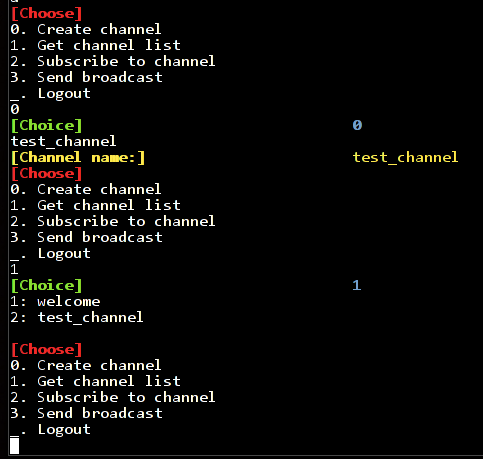
\includegraphics[width=0.65\textwidth]{di/3}
                \end{figure}

                \newpage

                The following diagram shows the steps required for \emph{post content editing}

                \begin{figure}[H]
                \caption{Post content editing activity diagram.}
                \centering
                \includegraphics[width=1\textwidth]{di/5}
                \end{figure}

                \newpage

                The following diagram shows the steps required for \emph{attachment creation}

                \begin{figure}[H]
                \caption{Attachment creation activity diagram.}
                \centering
                \includegraphics[width=1\textwidth]{di/6}
                \end{figure}

                \newpage

                The following diagram shows the steps required for \emph{content subscription}

                \begin{figure}[H]
                \caption{Content subscription activity diagram.}
                \centering
                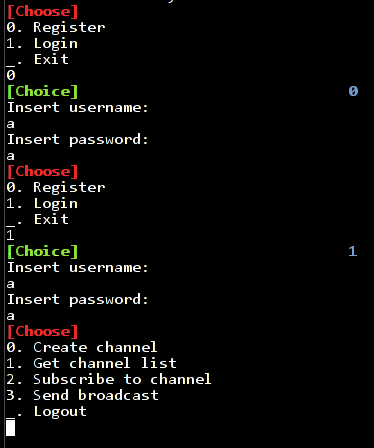
\includegraphics[width=1\textwidth]{di/2}
                \end{figure}

                \newpage

                The following diagram shows the steps that the \emph{forum system} must take in order to validate a permission bitset for a specific action.

                \begin{figure}[H]
                \caption{Recursive permission validation algorithm.}
                \centering
                \includegraphics[width=1\textwidth]{dn/0}
                \end{figure}

                \newpage
                \newpage

            \subsection{Class diagrams}

                \emph{Class diagrams} are created using UML.

                The \emph{Unified Modeling Language} (UML) is a general-purpose modeling language in the field of software engineering, which is designed to provide a standard way to visualize the design of a system.
                
                It offers a way to visualize a system's architectural blueprints in a diagram, including elements such as:

                \begin{itemize}
                    \item Any activities (jobs).
                    \item Individual components of the system.
                    \item And how they can interact with other software components.
                    \item How the system will run.
                    \item How entities interact with others (components and interfaces).
                    \item External user interface.
                \end{itemize}
                
                \begin{figure}[H]
                \caption{Database entities UML diagram.}
                \centering
                \includegraphics[width=1\textwidth]{uml/umldb}
                \end{figure}

                \newpage

                \begin{figure}[H]
                \caption{Server backend UML diagram.}
                \centering
                \includegraphics[width=1\textwidth]{uml/umlphp}
                \end{figure}

                \newpage
                \newpage

            \subsection{Sequence diagrams}                    

                The following diagram shows the interaction between \emph{forum users}, the \emph{subscription broker} and the \emph{content management} systen in order to manage subscriptions and generate notifications.

                \begin{figure}[H]
                \caption{Subscription/notification system sequence diagram.}
                \centering
                \includegraphics[width=1\textwidth]{uc/s1}
                \end{figure}

                \newpage

                The following diagram shows the interaction between the backend and the database.

                \begin{figure}[H]
                \caption{Backend-database interaction sequence diagram.}
                \centering
                \includegraphics[width=1\textwidth]{di/0}
                \end{figure}

                \newpage

                The following diagram shows the interaction between the backend and database stored procedures.

                \begin{figure}[H]
                \caption{Backend-stored procedures interaction sequence diagram.}
                \centering
                \includegraphics[width=1\textwidth]{di/4}
                \end{figure}

                \newpage

                The following diagram shows the interaction between the authentication system and the database.

                \begin{figure}[H]
                \caption{Authentication system-database interaction sequence diagram.}
                \centering
                \includegraphics[width=1\textwidth]{di/7}
                \end{figure}

                \newpage

                \newpage

            \subsection{Deployment diagram}

                A \emph{deployment diagram} in the Unified Modeling Language models the physical deployment of artifacts on nodes.

                The nodes appear as boxes, and the artifacts allocated to each node appear as rectangles within the boxes. Nodes may have subnodes, which appear as nested boxes. Device nodes are physical computing resources with processing memory and services to execute software, such as typical computers or mobile phones. 

                \begin{figure}[H]
                \caption{Deployment diagram for veeForum.}
                \centering
                \includegraphics[width=1\textwidth]{deployment}
                \end{figure}




\end{document}




